\chapter{Design}
\label{c:design}

This section presents the principle design of the monitoring system.
In the section \ref{ss:hardware} the components used are presented.
Section \ref{Dataflow} desctibes the functionalities and responsibilities of the system components.
In Section \ref{ss:network} the network topology and data-flow is discueed

\section{Hardware}
\label{ss:hardware}

This sectiondescribes the hardware used in the project. The setup consists of two distinct components: the artwork-tags, of which there are four, and one Phone that provides the interface to the user. The tag itself consists of 4 components:
\begin{enumerate}
	\item nRF52840 Microcontroler
	\item DWM3000 UWB Shield
	\item DHT22 temperature and humidity sensor
	\item MPU6050 accelerometer and gyroscope
\end{enumerate}

\subsection{Microcontroler}
The fundament of the artwork-tag is build by the nRF52840 DK microcontroller developed by Nordic Semiconductors. 
It is part of the nRF52 series of microcontrollers intended for development.
The nRF52840 DF is specialiezed for ble communication, for which it already includes the neccesary components.
It is compatible with the nRF52 Software Development Kit (SDK), also developed by Nordic Semiconductors.
The SDK makes it possible to use the ble functionalaties and to control the pins. It aslo includes implementations for a plethera of pin based protocols.
It contains 58 pins, 48 of which are data-pins and manage the power suply for additional modules, which includes 3.5 and 5 Volt supply pins.
32 of the pins are installed in the same way as the pins on the Ardruino uno, making it compatible with many peripherals that were designed with this common board in mind, such as the dwm3000.
The remaining ten pins are enough to attach the sensors to.
The nRF52840 DK includes a USB-B port that is used for Powersuply. Additionally it is connected to two pins and is used for UART-communication and for debugging.
The nRF52 was chosen since it was avaliable and previous projects have been done with it in compination with the DWM3000 shield.
As a result a lot of initial setup was already avaliable.

\subsection{UWB shield}
For communication between the tags as well as distance measurement the DWM3000 UWB-shield developed by Qorvo was chosen.
The DWM3000 is a commonly used device for research involving UWB \cite{coppens2022overview, leu2022ghost, stocker2022performance}.
It allows low level access, but includes an SDK written in C that makes a lot of the processes transparent to the user, if they wish.
The SDK uses the Serial Peripheral Interface (SPI) for communication between the shield and the microcontroler.



\subsection{Humidity and temperature sensor}

For humidity and temperature sensors I decided to use the DHT22(AM2302) produced by Guangzhou Aosong Electronic Co. \cite{AM2302}. 
It is a comonly used sensor in IoT monitoring systems \cite{ahmad2021evaluation}. 
The vendor claims a temperature range from -40\degree to 80\degree Celsius with a precision of 0.5\degree. 
\cite{ahmad2021evaluation} could experimentaly confirm that errors did not exceed 0.1\degree Celsius. 
They also concluded that the sensor is slow in detecting temperature change. 
This is also confrimed by the user manual \cite{AM2302}, that states a read-interval of less than 2s is not possible. 

The humidity sensor can detect the full range from 0\% to 99.9\% humidity, with an advertised maximum error of 2 percent-points \cite{AM2302}.
I could not find any research that confirmed or denied these claims.

The DHT22 sensor uses three pins from the microcontroler, two pins for power suply and ground and one for single-bus communication.
Since no SDK for this type of communication has been build for the nRF52 board series, it had to be implemented manually by reading the high and low voltage on the communication pin and, detecting headers and footers and parsing the binary messages. 
Dmitry Sysoletin published a project on github (\url{https://github.com/DSysoletin/nRF52_DHT11_example}) that handles the communication between an nRF52840 and a DHT11 sensor. 
Since the communications is mostly the same, I used his implementation, but changed the parsing of the actual data to fit the encoding used by the DHT22.

\subsection{Accelerometer and Gyroscope}
The MPU6050 sensor produced by InvenSense Incorporated provides accelerometer and gyroscope data.
The accelerometer reports the acceleration in the three cardinal directions in meters per second.
The Gyroscope reports the rotation around the threee euclidean axis in degrees per second.
In this project the accelermoterdata was not used, just the gyroscope.

The MPU6050 uses 4 pins, two for power suply and ground and two communication.
The Sensor communicates using the I2C protocoll, a serial synchronus communication system.
The microcontroller acts as the master and would in theory suport multiple workers on the same bus. 
Here only the MPU6050 uses I2C and is therefore the only worker.
While the nRF52 SDK does not supply a I2C API, it offers a Two Wire Interface (TWI) implementation that is compatible with the I2C protocoll.
It even used to offer MPU6050 specific support in the older SDK. 
I was able to port this older code to the current SDK.

\subsection{Tag technical plan}
The microcontroler builds the base of the Artwork-Tag. 
The other devices are attached to it over the avaliable pins.
In the nRF52 SDK each data pin is assigned an integer value. 
These often correspon with the name of the pin according to the nRF52830 DK manual, but not always.
I will use the names given in the manual to describe the pins.
Pins are the methods by which a microcontroller controls its peripheras.

Some pins are intended for power supply.
On the NRF52840 these pins are located in section P1, see table \ref{table:ArdruinoPins}.
The three VDD pins suply electricity with a Voltage of 3.5 Volts.
A secondary power supply that uses 5 Volts is also avaliable.
What voltage is needed depends on the periipheral.
In this case, the DHT22 runs on 3.5 Volts, while the MPU6050 is made for 5 Volts.
The P1 section also contains two ground pins, that need to be connected to the peripherals and a reset pin, so restart the microcontroler.
The last pin is not connected (N.C.).
There are additional ground pins in sections P4 and P24 of the board.

The other pins are called data pins.
By using voltage modulation these pins can transfer data and therefore be used for communication.
The nRF52840 has a I/O voltage of 3.3 Volt.
This means that a voltage of 3.3 Volt corresponds to a \textit{Logic high} and 0 Volts represents a \textit{Logic low}.
This allows the data pin to transfer communication in a binary encoding.
How a signal is interpreted is defined by the used communication protocol.
The MPU6050 for example uses the I2C protocol and uses 2 datapins.
This defines that one pin is used for a serial clock and the other pin transmits data.
For the data transmission the protocol defines what a package looks like.
This includes the start condition, the voltage characteristics that signal the beginning of a package, adressing, data encoding, acknowledgments and stop condition.

The DHT22 sensor does not use a given communication-protocol.
It uses one data-pin to report its sensor data.
How that data is encoded to high and low voltage is specified in the user manual \cite{AM2302} and has to implemented manualy.

The DWM3000 shield is mounted on the 32 pins ment for arduino one connections. 
All pins are forwarded and can be used by other devices, in a common ardruino-stackable style.
If they are data-pins they will share the data.
Table \ref{table:ArdruinoPins} shows which devices use which pins.
The only pin shared by multiple devices are power and ground pins.
The microcontroler suplies enough power to support this.

The sensors are attached to the same powersource and ground as the shield, but use different data-pins.
The DWM3000 leaves enough pins unused that both sensors could be attached to them.
Since it is not visible which pins the shield leaves free, I decided to use data-pins that are not attached to the DWM3000 in any way.
Table \ref{table:otherPins} shows how the sensors are connected to the remaining open pins.

\begin{table}[]
	\centering
	\begin{tabular}{l|l|l|l|l|}
		& Pin & \rotatebox{90}{DWM3000\phantom{.}} & \rotatebox{90}{DHT22}  & \rotatebox{90}{MPU6050\phantom{.}}   \\
		\hline \multicolumn{1}{|l|}{\multirow{10}{*}{\rotatebox{90}{P4}}}
		& P1.10  & \checkmark    &             &             \\
		\multicolumn{1}{|l|}{} & P1.11  & \checkmark    &             &             \\
		\multicolumn{1}{|l|}{} & P1.12  & \checkmark    &             &             \\
		\multicolumn{1}{|l|}{} & P1.13  & \checkmark    &             &             \\
		\multicolumn{1}{|l|}{} & P1.14  & \checkmark    &             &             \\
		\multicolumn{1}{|l|}{} & P1.15  & \checkmark    &             &             \\
		\multicolumn{1}{|l|}{} & GND    & \checkmark    &             &             \\
		\multicolumn{1}{|l|}{} & P0.02  &               &             &             \\
		\multicolumn{1}{|l|}{} & P0.26  & \checkmark    &             &             \\
		\multicolumn{1}{|l|}{} & P0.27  &               &             &             \\
		\hline \multicolumn{1}{|l|}{\multirow{8}{*}{\rotatebox{90}{P3}}}
		& P1.01  & \checkmark    &             &             \\
		\multicolumn{1}{|l|}{} & P1.02  & \checkmark    &             &             \\
		\multicolumn{1}{|l|}{} & P1.03  & \checkmark    &             &             \\
		\multicolumn{1}{|l|}{} & P1.04  & \checkmark    &             &             \\
		\multicolumn{1}{|l|}{} & P1.05  & \checkmark    &             &             \\
		\multicolumn{1}{|l|}{} & P1.06  & \checkmark    &             &             \\
		\multicolumn{1}{|l|}{} & P1.07  & \checkmark    &             &             \\
		\multicolumn{1}{|l|}{} & P1.08  & \checkmark    &             &             \\
		\multicolumn{1}{|l|}{} & P1.10  & \checkmark    &             &             \\
		\hline \multicolumn{1}{|l|}{\multirow{8}{*}{\rotatebox{90}{P1}}}
		& VDD    &               &             &             \\
		\multicolumn{1}{|l|}{} & VDD    &               &             &             \\
		\multicolumn{1}{|l|}{} & RESET  &               &             &             \\
		\multicolumn{1}{|l|}{} & VDD    & \checkmark    & \checkmark  &             \\
		\multicolumn{1}{|l|}{} & 5V     & \checkmark    &             & \checkmark  \\
		\multicolumn{1}{|l|}{} & GND    & \checkmark    & \checkmark  & \checkmark  \\
		\multicolumn{1}{|l|}{} & GND    & \checkmark    &             &             \\
		\multicolumn{1}{|l|}{} & N.C.   &               &             &             \\
		\hline \multicolumn{1}{|l|}{\multirow{6}{*}{\rotatebox{90}{P2}}}
		& P0.03  & \checkmark    &             &             \\
		\multicolumn{1}{|l|}{} & P0.04  & \checkmark    &             &             \\
		\multicolumn{1}{|l|}{} & P0.28  &               &             &             \\
		\multicolumn{1}{|l|}{} & P0.29  &               &             &             \\
		\multicolumn{1}{|l|}{} & P0.30  &               &             &             \\
		\multicolumn{1}{|l|}{} & P0.31  &               &             &             \\
		\hline 
	\end{tabular}
\caption{Adruino compatible pin assignment}
\label{table:ArdruinoPins}
\end{table}

\begin{table}[]
	\centering
	\begin{tabular}{l|l|l|l|l|}
		& Pin & \rotatebox{90}{DWM3000\phantom{.}} & \rotatebox{90}{DHT22}  & \rotatebox{90}{MPU6050\phantom{.}}   \\
		\hline \multicolumn{1}{|l|}{\multirow{8}{*}{\rotatebox{90}{P6}}} 
		& P0.00  &               &             &             \\
		\multicolumn{1}{|l|}{} & P0.01  &               &             &             \\
		\multicolumn{1}{|l|}{} & P0.05  &               &             &             \\
		\multicolumn{1}{|l|}{} & P0.06  &               &             &             \\
		\multicolumn{1}{|l|}{} & P0.07  &               &             &             \\
		\multicolumn{1}{|l|}{} & P0.08  &               &             &             \\
		\multicolumn{1}{|l|}{} & P0.09  &               &             &             \\
		\multicolumn{1}{|l|}{} & P0.10  &               &             &             \\
		\hline \multicolumn{1}{|l|}{\multirow{18}{*}{\rotatebox{90}{P24}}} 
		& P0.11  &               &             & \checkmark  \\
		\multicolumn{1}{|l|}{} & P0.12  &               &             & \checkmark  \\
		\multicolumn{1}{|l|}{} & P0.13  &               & \checkmark  &             \\
		\multicolumn{1}{|l|}{} & P0.14  &               &             &             \\
		\multicolumn{1}{|l|}{} & P0.15  &               &             &             \\
		\multicolumn{1}{|l|}{} & P0.16  &               &             &             \\
		\multicolumn{1}{|l|}{} & P0.17  &               &             &             \\
		\multicolumn{1}{|l|}{} & P0.18  &               &             &             \\
		\multicolumn{1}{|l|}{} & P0.19  &               &             &             \\
		\multicolumn{1}{|l|}{} & P0.20  &               &             &             \\
		\multicolumn{1}{|l|}{} & P0.21  &               &             &             \\
		\multicolumn{1}{|l|}{} & P0.22  &               &             &             \\
		\multicolumn{1}{|l|}{} & P0.23  &               &             &             \\
		\multicolumn{1}{|l|}{} & P0.24  &               &             &             \\
		\multicolumn{1}{|l|}{} & P0.25  &               &             &             \\
		\multicolumn{1}{|l|}{} & P1.00  &               &             &             \\
		\multicolumn{1}{|l|}{} & P1.09  &               &             &             \\
		\multicolumn{1}{|l|}{} & GND    &               &             &             \\
		\hline
	\end{tabular}
\caption{Non-Adruino compatible pin assignment}
\label{table:otherPins}
\end{table}


\section{Architecture}
\label{ss:dataflow}

In order to discuss how the dataflow works, first the section \ref{ss:responsibility} will establish what services are implemented in each part of the system.
The section \ref{ss:dataflow} will explain what triggers events and how they are handled inside the system.

\subsection{Responsibilities}
\label{ss:responsibility}
The system consists of the tags, the sensor network and the phone.
These parts all have their own responsibilities.

\textbf{Tag:} 
The tag is responsible to manage its sensors. 
It has to do correct setup and converts its output into a understanable form.
The tag can performe ranging with all its neighbours.
Additionaly the tags are responsible to search for networks to join, and react aprobiatly to network request, be those queries for sensor data, ranging requests or network managment jobs. 
The tags provide a unique, secure universal identifier, to be used by queries or the network.
How this is done is part of the certify project and will not be discussed in this thesis.
The tag is also responsible for its own power managment.
This is not the focus of this thesis and will only be mentioned when relevant.
A guideline on powermanagment will not be provided here.

\textbf{Network:} The network is responsible to keep track of all tags taking part in the network. 
It offers a joining protocol for new devices and remains stable when devices leave or become unavaliable. 
It offers the possibility for phones to connect to the network. 
It ensures quieries from phones get transported to the correct tag and the answers to the correct phone.
It ensures a network topology that corresponds to a graph that is at least 3-connected.
On request it returns a list of connected devices to the phone.

\textbf{Phone:} The phone connects to the network via the provided method.
It offers a graphical user interface (GUI) to be used by the driver.
The GUI offers a method for the driver to set the acceptable ranges for all sensor data.
Additionaly it offers a method to set query intervals-length.
The phone is responsible to query sensor data for each tag and masurement once in each interval.
The phone has to evaluate the answer.
The phone has to report the results to the driver using the GUI.
If a parameter falls outside of the acceptable range for its type, the phone is responsible to alert the driver to this fact.

The certify project also plannes to collect the sensor data on remote servers using a 4G connection.
The plan is to equip each tag with antennas to allow it to send the data directly to the server itself.
Since this is not a part of this thesis, the responsibility for the tag to do this was not added to a list.
A known problem with this plan is, that a 4G connection is not always possible.
Since small tags have very limited memory, the plan to store the sensor data on the tag is not pheasible.
If the setup presented in this thesis is used, it would allow for the storage of the data on the phone, which has a much larger memory.
This again was not added, since it is not part of this thesis.

\subsection{Dataflow}
\label{ss:dataflow}

\begin{figure}[ht!]
	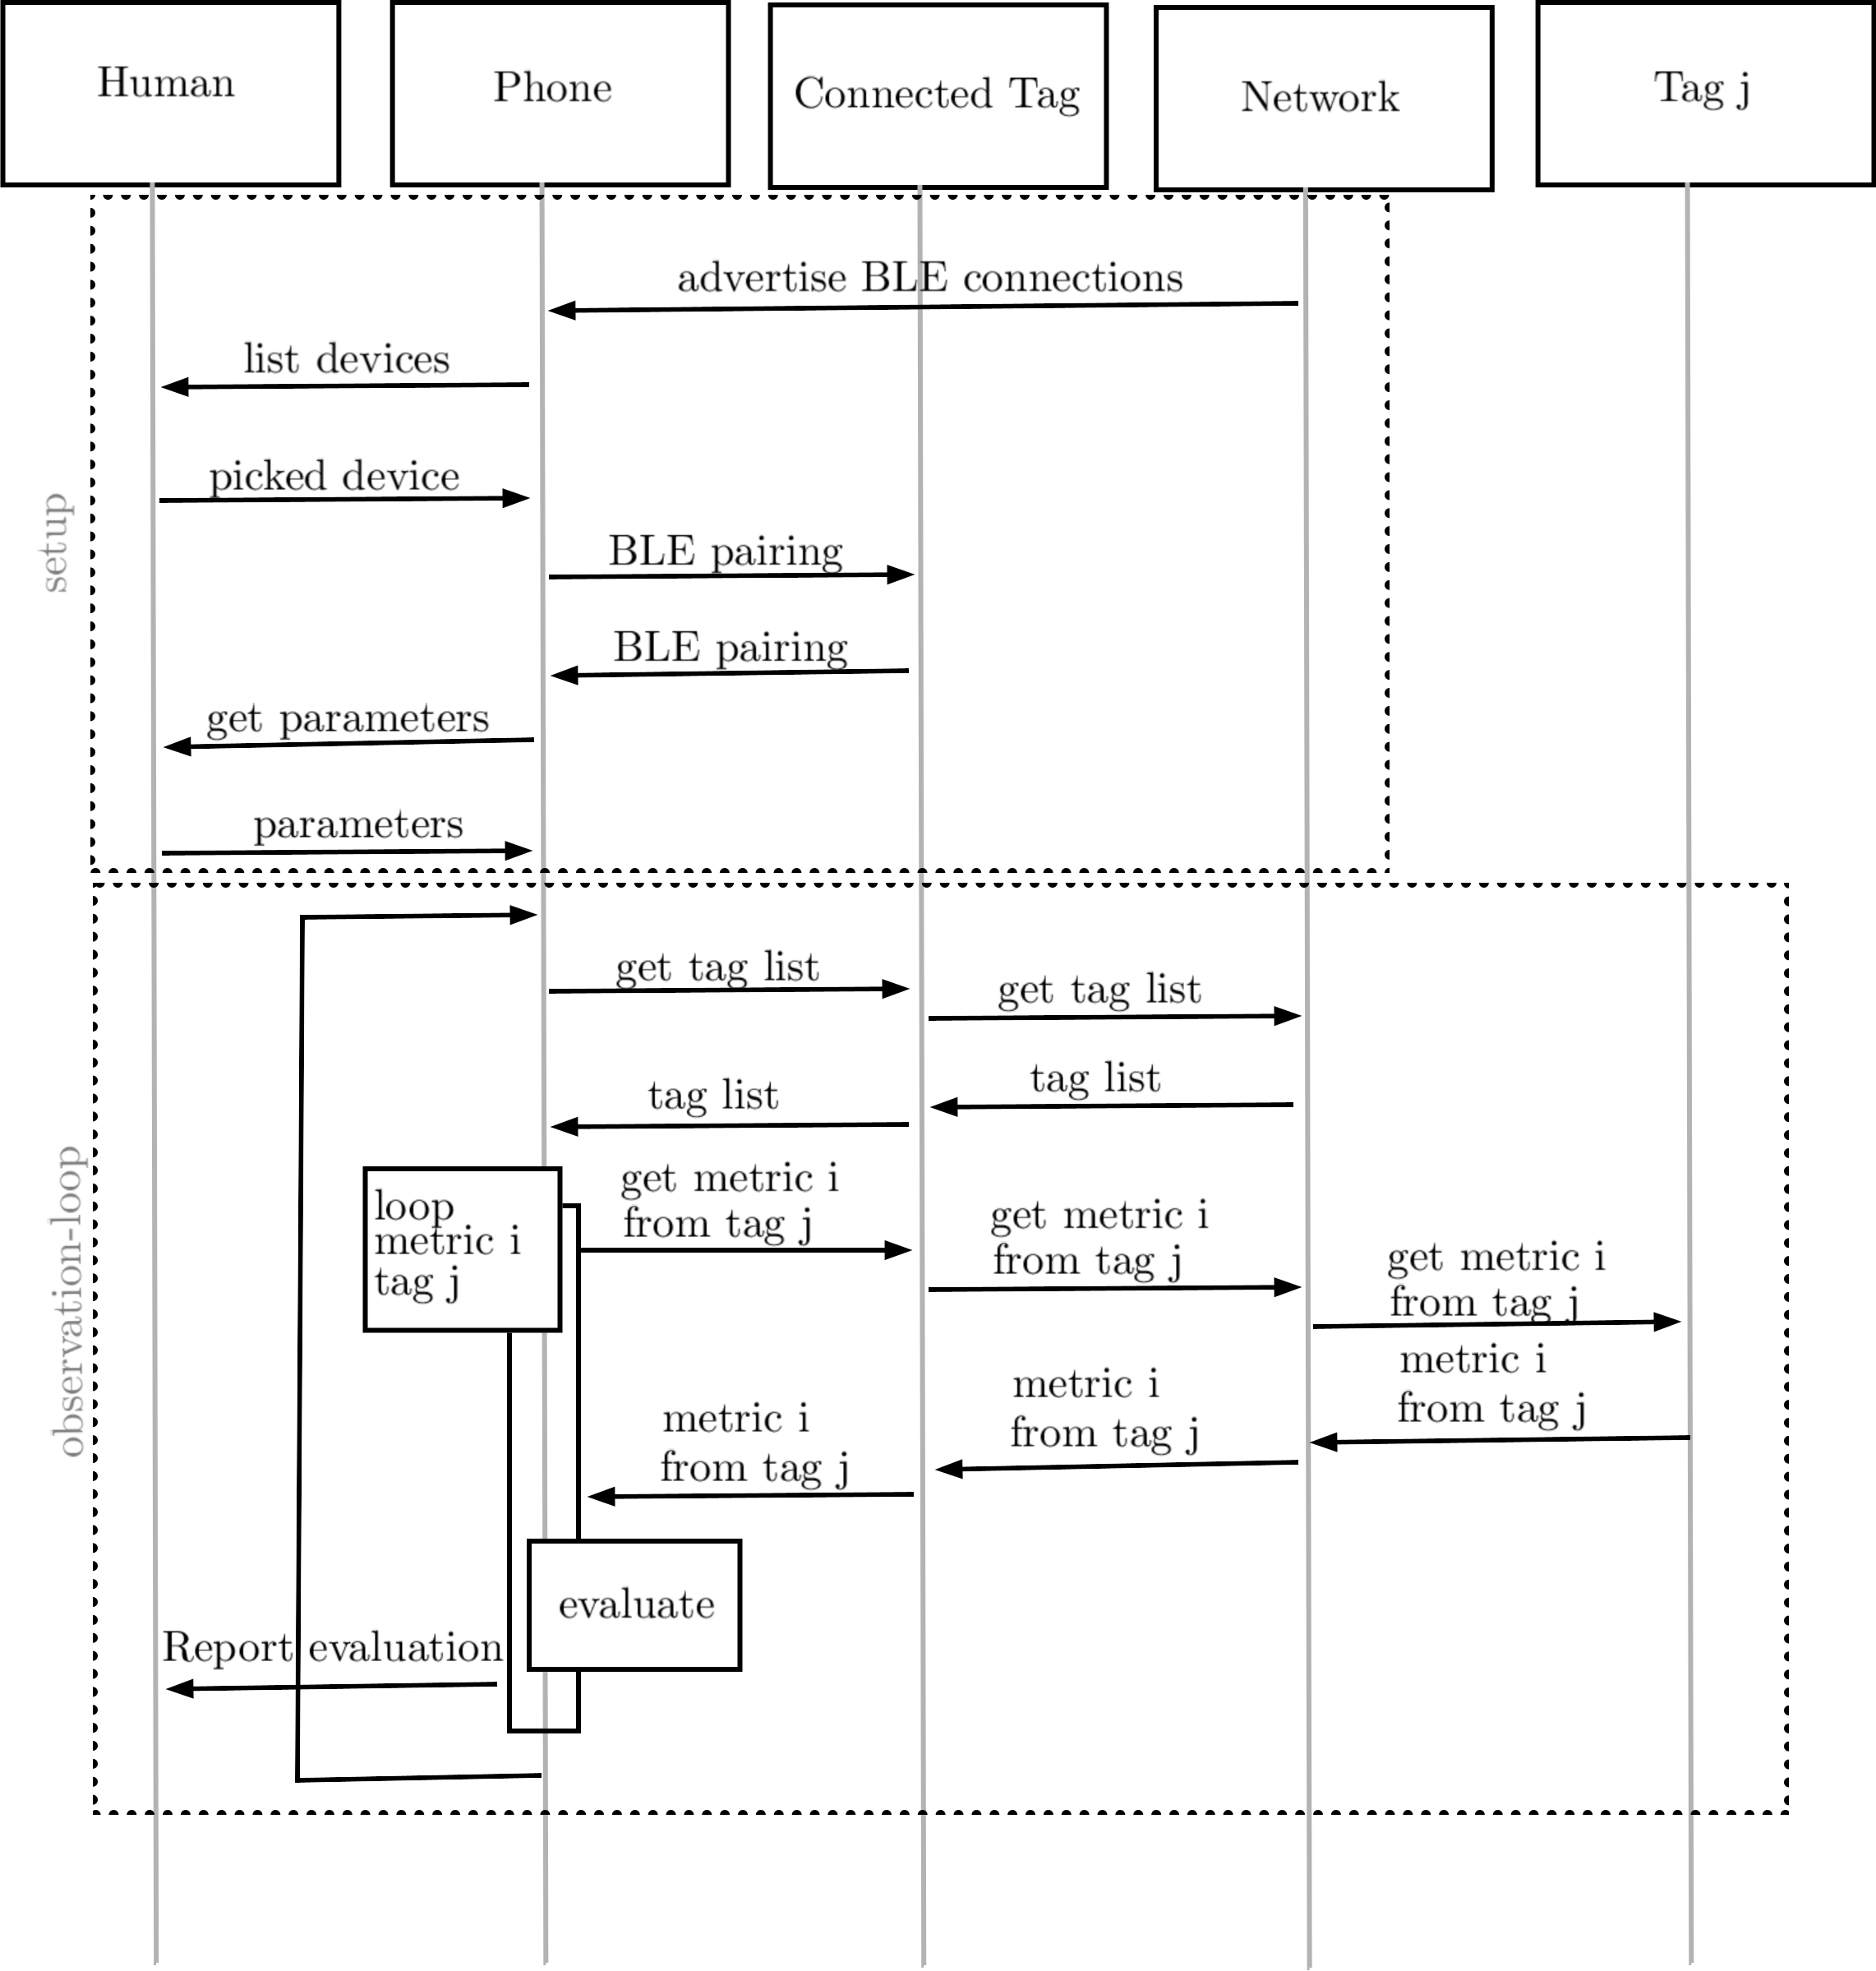
\includegraphics[width=\linewidth]{graphics/schematics/obervation_loop.png}
	\caption{Sequence diagram of setup and oberservation loop. Setup is performed once, oberservation loop repeats until stopped.}
	\label{f:observation_loop}
\end{figure}

How a tag connects to the network is described in the section \ref{s:network}.
Figure \ref{f:observation_loop} shows a sequece diagram ob the setup and main observation loop of the system.
On the top the communicating parts are listed.
\begin{itemize}
	\item Human is the driver of the truck
	\item Phone is the phone used by the Human
	\item Network consists of all the tags that are used and the network they build.
	\item Connected Tag is part of this network, but is listed seperatly. It represents the tag that is communicating to the phone
	\item Tag j is also part of the Netowrk. It represents the tag that is queried during the observation loop
\end{itemize}
Phone and Human communicate by using a GUI. Phone and Connected Tag commuincate using BLE. Every communication inside the network happens using UWB. This includes the communication between the Connected Tag, the network and Tag j. \\
When the phone wants to connect to the network, it looks for advertised BLE devices.
It then displays the devices to the user and lets him pick one.
The phone then pairs to the chosen tag, making it the connected tag and the phones connection to the network of tags.
Once connected to the network, the phone will promt the human to enter the parameters.
These consist of:
\begin{itemize}
	\item Upper and lower limit for sensor data, like temperature and humidity
	\item Maximal displacement value for distance and gyro. These values represent the maximal difference in registered values that is allowed for positional measurements.
	\item Time between measurements. This gives the time period that will pass between measurements for each device and measurement type.
\end{itemize}
Once the parameters chosen, the user can start the observation.\\
Each iteration of the observation loop begins with a call to the network for a list of all tags currently in the network.
Since the tag network is a dynamic sensor network, the tags in the network can theoretically change. 
In practice this should onyl happen, when artwork is unloaded or if a tag becomes faulty.
The request for the list is transmitted to the connected tag ober BLE, which than queries the network for all conected devices.
The responde is returned to the Phone.
The phone then starts a nested loop, iterating over the list of tags and the list of metrics caputred by the system.
For each measurement and tag combination (i,j) the phone contacts the connected tag for the value, which in turn queries the network.
Once the message has arrived at the tag j, tag j gets measurement i. In case of sensors this intails contacting the sensor and requesting a value.
If metric i is a distance measurement, tag j will commence a two-way ranging operation over UWB with all its registered neighbours and will report the list of distances, together with the tag-adresses they correspond to.
Metric i is then transported over the network back to the connected tag and finaly to the phone.
The phone must then evaluate the retrieved data. \\
During the evaluation process, the phone creates an evaluated measurement, and marks it as problematic or unproblematic.
What the evaluation looks like depends on the metric.
\begin{itemize}
	\item For most metrics, like humidity and temperature, the evaluated measurement is equivalent to the received measurement. It is then checked, if the measurement falls into the aceptable measurement parameters, set by the human.
	If it does not, the evaluated value is marked as problematic.
	\item Some metrics require comparisment to the previous data. The gyroscope reports the current orientation of the tag.
	This is then compared to all previous measurements and the maximal angular difference forms the evaluated measurement.
	If the evaluated metric is bigger then allowed by the set parameters, the measurement is marked as problematic
	After evaluation the original measurement is added to the list of previous measurements.
	\item The distance measurement has a unique evaluation process, which is describbed in section \ref{ss:distance_eval}.
\end{itemize}
Once the data evaluation is done, the evaluated measurement is presented to the user over the GUI, together with the adress of the tag it belongs to.
If the evaluated measurement is problematic, the driver it alarmed.


\subsubsection{Distance evaluation}
\label{ss:distance_eval}
The goal of the distance evaluation is to build a working model of where every tag is.
To achieve this, a quadratic program is solved, to get the coordinates of all tags.
The steps to do this are as follows:
\begin{enumerate}
	\item Get a list of all current tags, $T:=\{ t_1, t_2, ... \}$.
	\item For each tag, get the last known distance measurements and put it into a set $S_D:=\{ (t_i, t_j, d_{ij}) \} $, where $t_i$ is the tag which measured, $t_2$ the tag that was measured to and $d_{ij}$ the distance measured.
	\item If a tag has no distance measurements, remove it from the list.
	\item Assign each tag $t_i$ a position in a 3D coordinate system, $(x_i,y_i,z_i)$
	\item Pick one random tag $t_{o}$.
	\item Set the values $x_{o},y_{o},z_{o}$ all to 0.
	\item Create the objective function: $L(X,Y,Z) = \sum\limits_{t_i, t_j, d_{ij} \in S_D}|(x_i-x_j)^2+(y_i-y_j)^2+(z_i-z_j)^2-d_{ij}^2|$. For x,y and z use variables for all but the six values set in step (6).
	\item Solve the quadratic program consting of the Objective function L and no constrains.
\end{enumerate}
Quadratic Programs in general are NP-Hard, but Quadratic Programs with a convex function can be solved efficiently.
$(a-b)^2$ and $c$ are convex functions.
The sum uf a convex function is always a convex function.
The objective function in (7) only sums up convex functions and is therefore convex itself.
The quadratic program can therefore be solved efficiently.\\
By setting the values of tag $t_{o}$ to zero, the results of the quadratc function becomes grounded.
It is not strictily nessecary, but without it the returned solution could have values anywhere in the Euclidean space.
by setting one tag to the coordinates at theo origin, the solution will place the other tags near that region.
There are still an infinte amount of solutions to this quadratic function, since all solutions can be roatated around any axis and still return the same objective function.

\begin{figure}[ht!]
	\begin{subfigure}{.4\linewidth}
		\centering
		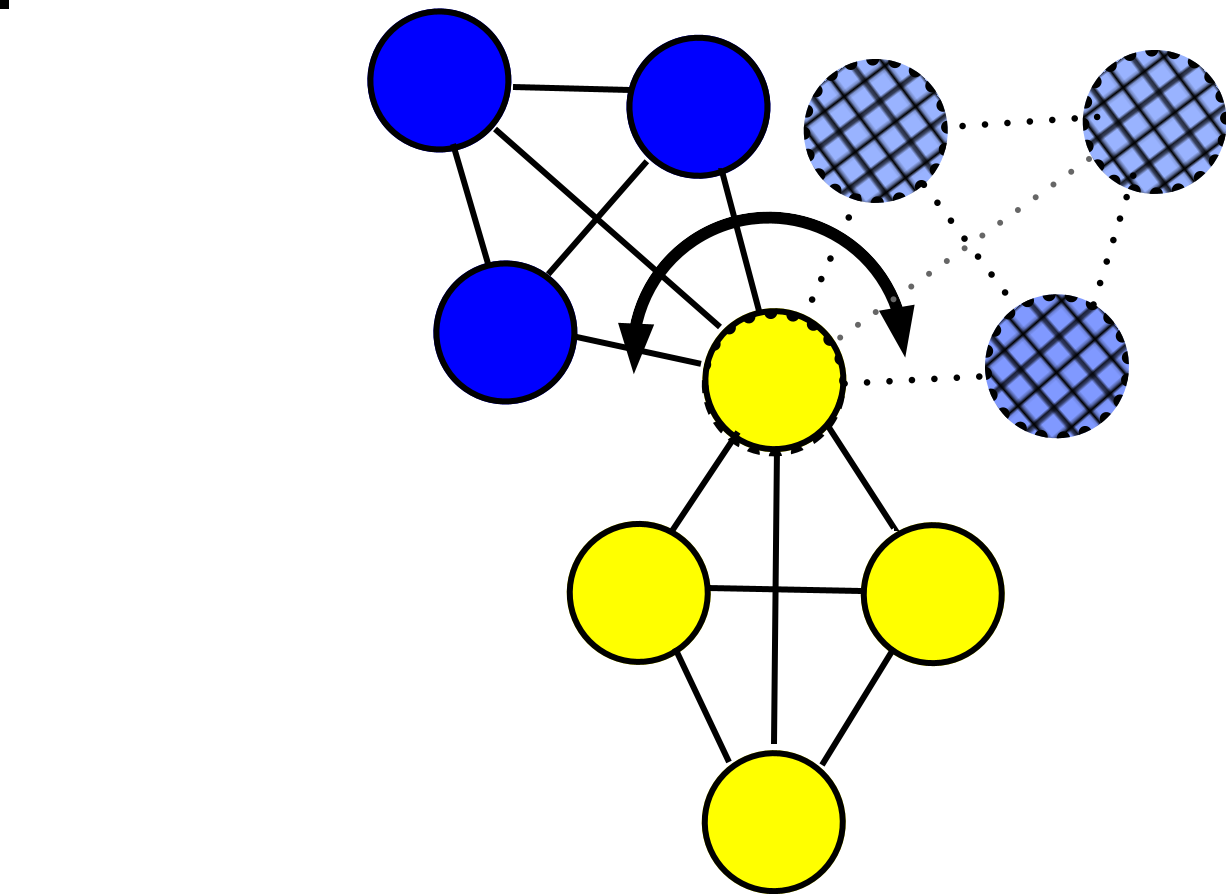
\includegraphics[height=150px]{graphics/schematics/connected_dots.png}
		\caption{3-edge connected graph}
	\end{subfigure}
\hspace{1cm}
	\begin{subfigure}{.4\linewidth}
		\centering
		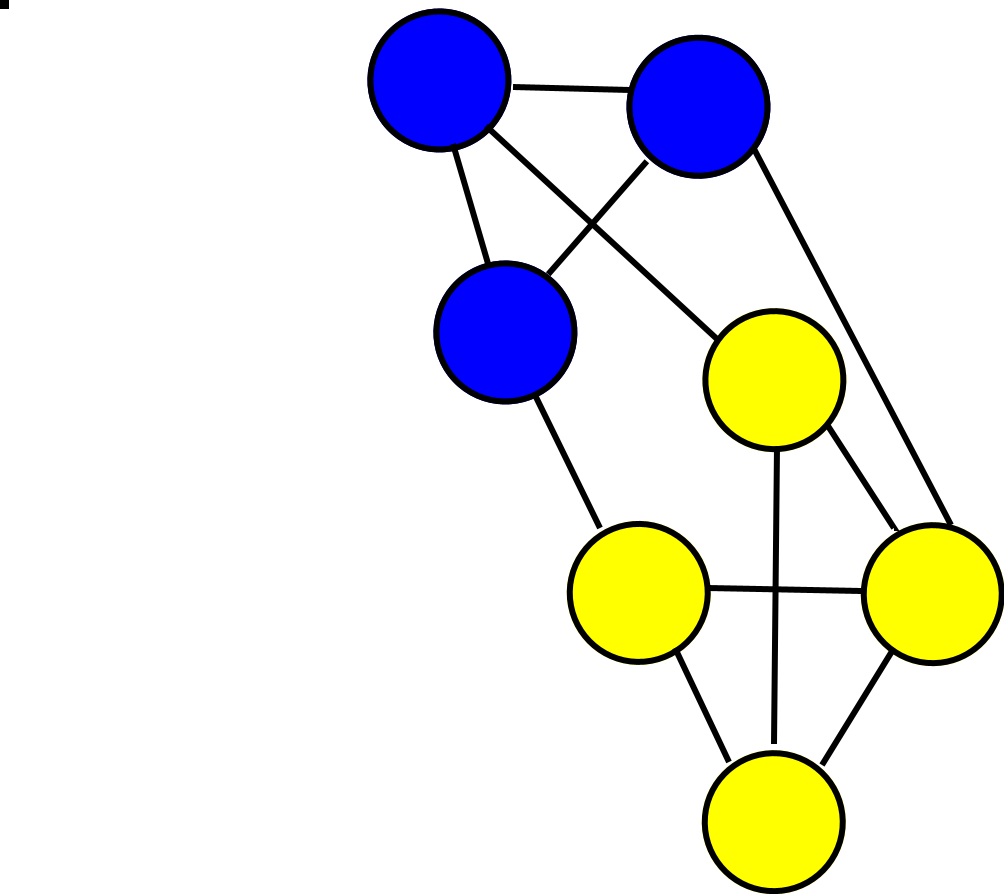
\includegraphics[height=150px]{graphics/schematics/connected_dots_k_connected.png}
		\caption{2 connected graph}
	\end{subfigure}
	\caption{ Left: Five dots, all having at least two connections, still blue can move independently. Right: minimal 2-connected graph, no movement possible. }
	\label{f:connected_dots}
\end{figure}

For a point to be clearly placed in Euclidean space, three distances to other points have to known.
This alone is not sufficient to insure a unique results.
The left of Figure \ref{f:connected_dots} illustrates this point in two-dimensional space.
Every circle is connected to two others, still the blue circles can move without the whole figure moving.
What is needed to keep every point static is for known distances and tags to build a four-connected graph (three in two dimensions).
The left of Figure \ref{f:connected_dots} shows a sollution of the problem on the right by creating a three-connected subgraph.

Once the coordinates for all tags are found, they are compared to previous results.
For each tag the phone calculate by how much it has moved.
The evaluated measurment is the distance of the tag that has moved the most.
If the evaluated measurement is larger then the maximal allowed displacement, the measurement is problematic.



\section{Network}
\label{s:network}

For the presented network to work, tags need to be ranked.
This means that for each tag pair $i,j$, one can either say that $rank(i)<rank(j)$ or $rank(j)<rank(i)$.
To achieve this, the universal unique identifiers are used.
No matter what form the UUID has, it can be converted to an integer, by simply interpreting its binary code as one.
Since the UUIDs are unique, no to tags will have the same resulting integer.
When refering to the rank of a tag in this section, the integer representing the UUID is intended.

The tags inside the truck, while not connected to a phone, form a dicentralized mesh using UWB for communication.
Each tag keeps two list, a list of known devices and a list of neighbours.
When a new tag joins the network, it sends a joining request over UWB, containing its universal unique id (UUID), using a weak signal.
All tags in the network that receive this request add the new device to their list if known devices. 
If the new devices also has a heigher rank, they additionaly add it to their list of neighbours.
They then answer by sending their own UUID and adress back to the new tag.
By waiting an amount of time that correlates with their UUID, the tags in the network can ensure, that their answers don't overlap.
The new tag adds the received adresses and UUIDs to its known device list. If the rank of the added tag is also has a higher rank then the new tag, it will add it to the list of neighbours.
If the new tag now has four neighbours, it stops. Otherwise it will repeat the process with a incresasingly stronger signal, until it has either found four tags with higher rank or reached maximum signal strength.
Afterwards it starts addvertising its BLE connection.
This concludes the network joining process.


A user with a phone can connect to any of the advertised BLE connection.
Once that happens, the tags in the tracks will switch from their dicentralized mesh to a star-topology, with the connected device serving as the coordinator.
The coordinator will inform all tags about its new status, by sending a message using a strong UWB signal.
The tags will then acknowledge this message in order of rank.
The tags in the network will still keep their stored neighbours and known devices.
The coordinator records a list of all acknowledgemtns, thus creating a list of all devices in the network.


The phone can request the list of all tags from the coordinator.
The phone can now also query the tags in the truck by sending the query to the coordinator over BLE, which then will pass it directly to the apropriate tag using BLE.
For all sensor data, this is a simple call and response request. \\
If a distance measurement is queried, the tags takes the following steps:
\begin{itemize}
	\item It conducts a UWB two-way ranging session with each tag in the neighbour list.
	\item It reports those results to the coordinator tag.
	\item It orders all received distances.
	\item It keeps the tags with the four lowest distances and deletes the rest from the neighbour list.
\end{itemize}
The first time a distance is requested, the tag will perform more ranging sessions then necesary to build a 4-connected graph.
Afterwards it only perform ranging with four other tags, unless a new device was added.
If a ranging session does not report a result, because a tag left or became unavaliable, the tag adds ads the tag with the shortest previously measured distance and higher rank from the list of known devices back intro the list of neighbours.


This design mirrors the algorithm proposed by \cite[khan2007simple] and presented in section \ref{ss:k_connected_explained}.
It creates an approximation of a minimaly weighted k-connected subgraph, based on the measured distances.
This is allowed, since the distances are in euclydean space, which when mapped to a graph forms a metric graph.
As discussed in section \label{ss:distance_eval}, a four-connected graph is needed to uniquly identify the position of each tag.
The graph should be minimaly weighted, so that measurements are between tags that are as close as possible to each other.
This reduces the multipath effect and theirfore increases precision.


If the tags are not connected to a phone and report their data to a remote server, they can still use the same distance-measurement, to approximate the k-connected subgraph.
The quadratic program can then be calculated on the server.